\chapter{Integracja układu FPGA z dronem}
Opisana w poprzednim rozdziale architektura sprzętowa dotyczyła dwóch algorytmów, które mogą funkcjonować niezależnie od siebie. Ostatecznie jednak istnieje jeszcze najwyższa warstwa logiczna, która pozwala wykorzystać je jak najlepiej, oraz odpowiada za komunikację z dronem.

\section{Konstrukcja drona}
Poniżej opisane są parametry wykorzystywanej maszyny:
\begin{itemize}
	 \item typ obiektu: hexacopter (rama DJI F550),
	 \item rodzaj śmigieł: wzmocnione śmigła o oznaczeniu 9050, czyli o średnicy śmigła równej $9.0"$ ($~22.86$cm) oraz skoku śmigła $5.0"$ ($~12.7$cm).,
	 \item silniki: DJI 2312/960KV sterowane kontrolerami 420 LITE
	 \item zasilanie: czterokomorowa bateria LiPo o nominalnym napięciu $14.8$V (maksymalnym $16.8$V) oraz o pojemności $6450$mAh,
	 \item kamera: Xiaomi Yi,
	 \item gimbal: Tarot T-2D,
	 \item aparatura radiowa: FrSky Taranis X9D Plus,
	 \item odbiornik: FrSky X8D,
	 \item autopilot: 3DR Pixhawk.
\end{itemize}
\subsection{Autopilot}

Każdy dron byłby bezużyteczną konstrukcją, gdyby nie serce maszyny - tzw. autopilot. W tym przypadku postanowiono wykorzystać urządzenie Pixhawk. Jest to zgodny ze standardami przemysłowymi moduł na otwartej licencji, stworzony przy współpracy z 3D Robotics oraz ArduPilot Group. Posiada następujące parametry:
\begin{itemize}
	\item procesor Cortex-M4F taktowany zegarem 168 MHz,
	\item sensory: trzyosiowy akcelerometr, żyroskop, kompas magnetyczny, barometr i zewnętrzny GPS,
	\item slot na kartę microSD,
	\item możliwość połączenia peryferiów (interfejsy: UART, I2C, CAN),
	\item 14 wyjść PWM (8 głównych z zabezpieczeniami + 6 dodatkowych).
\end{itemize}

\begin{figure}[h]
	\centering
	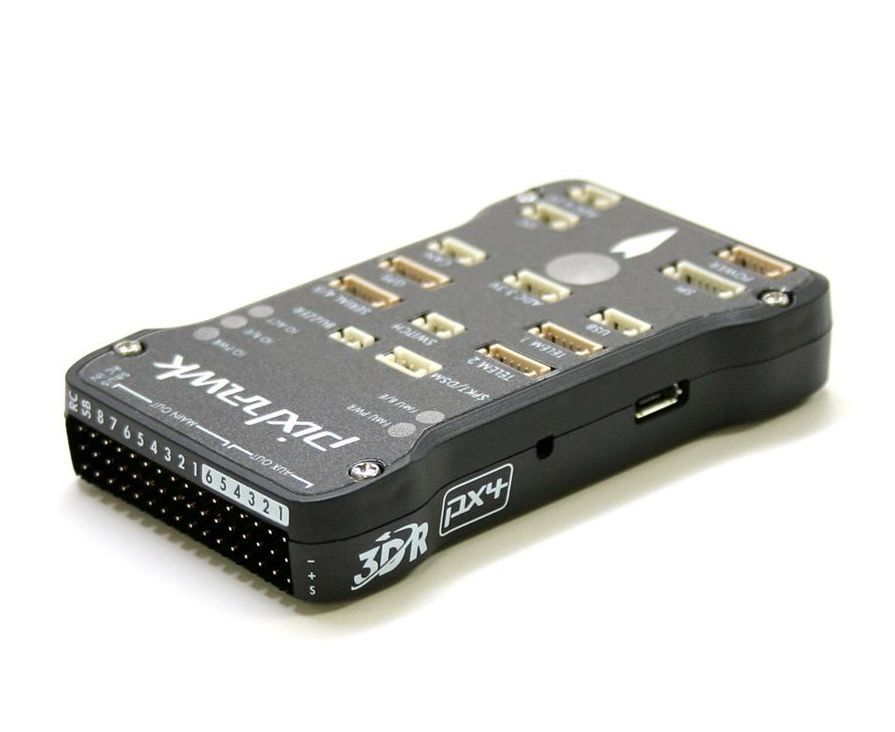
\includegraphics[width=8cm]{5_pixhawk.jpg}
	\caption{Autopilot Pixhawk - widok na panel główny oraz we/wy PWM}
	\label{fig:pixhawk}
\end{figure}

Powyższy sprzęt jednak nie jest w pełni skonfigurowany do pracy po wyjęciu z pudełka - szczególnie, że jako uniwersalny produkt, bywa montowany na konstrukcjach o szerokim rozrzucie parametrów. Może zapewnić sterowanie kopterom, samolotom modelarskim oraz nawet łazikom. W przypadku dwóch pierwszych grup konfiguracja wiąże się ze zdefiniowaniem odpowiedniej liczby śmigieł i ich rozstawienia, typu aparatury radiowej oraz zewnętrznych urządzeń geolokalizacyjnych. Tę dość dużą elastyczność mogą zapewnić dwa główne systemy, które są wczytywane z pamięci SD i pracują w czasie rzeczywistym. Dedykowany, PX4 Flight Stack jest stworzony przez twórców modułu, oraz ArduPilot Copter (ArduCopter) - niezależny, otwarty system, który został dostosowany do platformy Pixhawk z wykorzystaniem dostępnych narzędzi deweloperskich. Ze względu na większą bazę użytkowników i dojrzałość projektu, wybrano drugie rozwiązanie.

\begin{figure}[h]
	\centering
	\captionsetup{justification=centering,margin=1cm}
	\hspace*{0cm}
	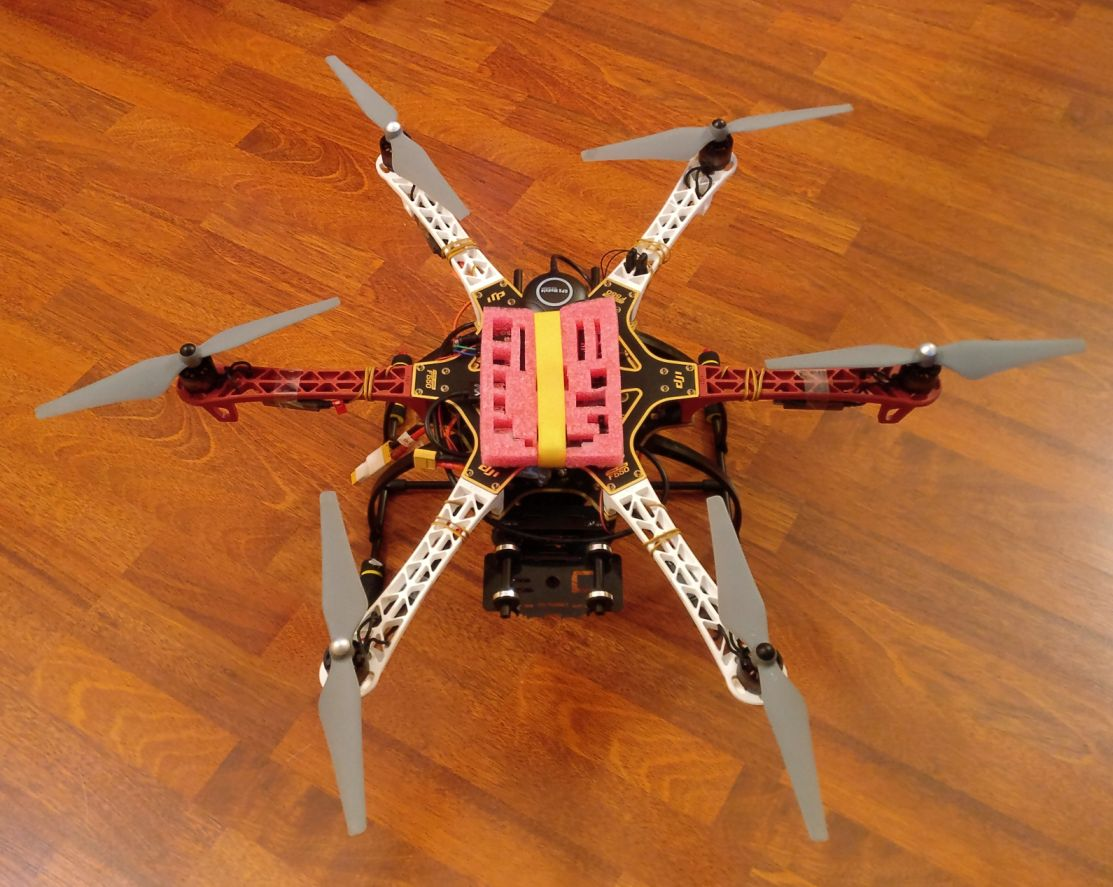
\includegraphics[width=14cm]{5_drone_photo.jpg}
	\caption{Zdjęcie przedstawiające w pełni wyposażonego drona. Pod gąbką ochronną skrywa się układ PYNQ}
	\label{fig:drone_photo}
\end{figure}

\subsection{Propagacja sygnałów}
Zbudowanie drona w oparciu o gotowe komponenty nie jest zadaniem skomplikowanym. Jednak w momencie, gdy doszły elementy zapewniające jego autonomizację, należało dokładnie przemyśleć jego przebudowę. Schemat \ref{fig:architecture} przedstawia architekturę sygnałową.
\begin{figure}[]
	\centering
	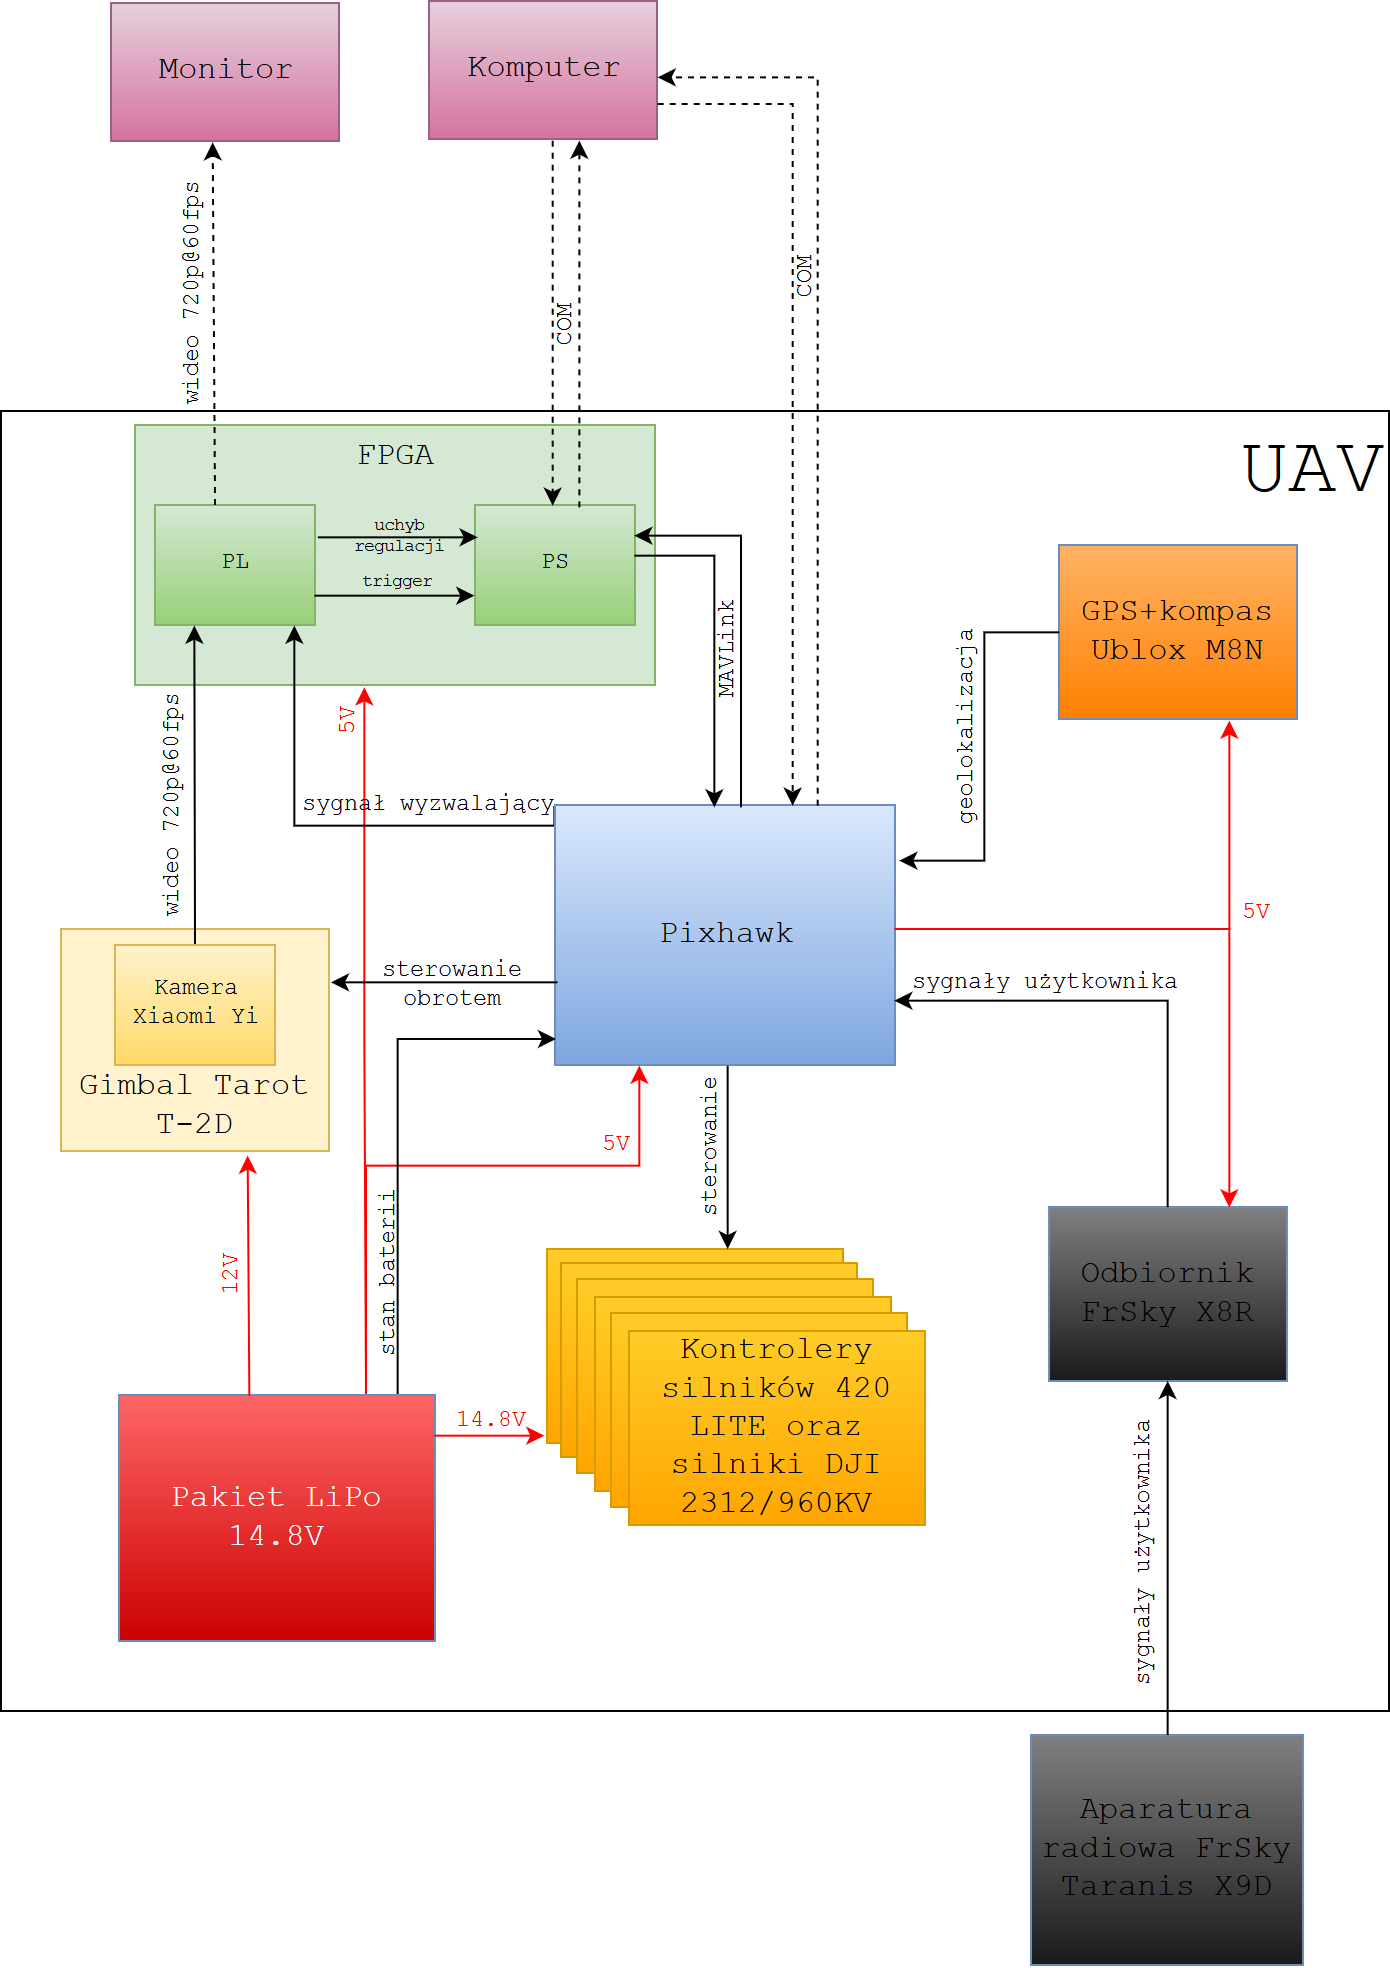
\includegraphics[width=14cm]{5_drone_architecture.png}
	\caption{Architektura sygnałowa tworzonego projektu}
	\label{fig:architecture}
\end{figure}

\section{Zdalne uruchomienie pracy systemu}

Początkowo stworzono (i ostatecznie pozostawiono) możliwość rozpoczęcia pracy z wykorzystaniem jednego z przełączników na płycie PYNQ, gdyż prace nad projektem wymagały dość częstego uruchamiania algorytmu jeszcze bez udziału drona. Jednak lot maszyny lub nawet jego start praktycznie wyklucza fizyczny dostęp do układu FPGA, dlatego koniecznością stało się zdalne wyzwolenie pracy algorytmów. Sygnał wyzwalający nosi nazwę \textit{trigger\char`_algorithm}.

Podczas lotu maszyny użytkownik ma pod ręką jedynie aparaturę radiową, z poziomu której może jednak w dość prosty sposób wystawiać sygnały. Aparatura jest bowiem wyposażona w szereg konfigurowalnych przełączników analogowych i cyfrowych. Ponadto, zdolna jest do transmisji 16 kanałów - przy czym do kontroli podstawowych funkcji drona wykorzystuje się zaledwie 4. Wybrano zatem jeden z pozostałych dostępnych kanałów, któremu przypisano funkcję trzypoziomowego przełącznika obecnego na panelu urządzenia radiowego.

Sparowany z aparaturą odbiornik wysyła wszystkie dane po jednym zestawie przewodów w formie PPM (ang. Pulse Position Modulation). Taki sygnał musiałby być zdekodowany w układzie FPGA do uzyskania użytecznej wartości. Proces dekodowania rozwiązuje jednak autopilot, który na podstawie 16-kanałowego PPM wystawia znacznie prostsze sygnały PWM (ang. Pulse Width Modulation) m.in. do kontroli silników. Co więcej, Pixhawk umożliwia przypisanie reszty kanałów transmisyjnych do pomocniczych wyjść PWM. Rozwiązanie to znalazło zastosowanie chociażby w ustawieniu wartości zadanych serwomechanizmom odpowiedzialnym za pracę gimbala kamery.

Ostatecznie kwestią niejasną pozostała szerokość pulsu, który miałby wyzwolić działanie algorytmu. O ile dla typowego sygnału PWM powinien on wynosić od 1ms do 2ms, to zdecydowano się ustalić wartość dla każdej z trzech pozycji przełącznika. Zastosowano w tym celu analizator logiczny ILA wbudowany w środowisko Vivado i stworzono prosty licznik, na którym stosuje się następujące operacje:
\begin{itemize}
	\item kasowanie na zboczu narastającym sygnału wejściowego,
	\item inkrementację podczas aktywnego stanu sygnału,
	\item przypisanie tej samej wartości w każdym innym przypadku.
\end{itemize}

Logika pracuje na zegarze \textit{calc\char`_clk} $=100$MHz i dla poszczególnych wartości przełącznika na aparaturze radiowej wartości licznika są przedstawione w poniższej tabeli. Pokazuje ona, że zakres długości pulsu nie odstaje od normy typowego sygnału PWM, mimo że jest nieco zawężony.

\newcolumntype{P}[1]{>{\centering\arraybackslash}p{#1}}
\begin{table}[h]
	\centering
	\begin{tabular}{|P{4cm} |P{3cm} |P{4cm}|}
		
		\hline
		\rowcolor{lightgray} Pozycja przełącznika & Wartość licznika & Długość pulsu [ms]  \\ 
		-1	& 109000 & 1.09	\\ 
		\hline
		0	& 149000 & 1.49 \\ 
		\hline
		1	& 189000 & 1.89 \\ 
		\hline
	\end{tabular}
	\caption{Szerokości pulsu PWM dla przełącznika odpowiedzialnego za start algorytmu}
	\label{tab:RFswitch}
\end{table}

Na tej podstawie określono, że warunkiem koniecznym do rozpoczęcia algorytmu będzie wystąpienie dwóch kolejnych pulsów o szerokości przynajmniej 1.8ms (górny limit przezornie ustawiono na 2ms). Analogicznie, zakończenie pracy algorytmu i powrót do ustawień domyślnych będzie miał miejsce dla dwóch pulsów o wartości spoza zakresu.

\section{Kontrola nad pracą algorytmów MeanShift oraz HoG+SVM}

Najwyższa warstwa w części programowalnej FPGA, łącząca pracę obu algorytmów, zarządza sygnałami mogącymi je niezależnie uruchomić. Zanim jednak przyjdzie na to pora, zadaniem maszyny stanu jest oczekiwanie na informację o gotowości drona, tj. ustabilizowaniu pozycji w powietrzu. 

Po otrzymaniu takiego sygnału kolejnym etapem jest pierwotna detekcja postaci. Wykorzystywany w tym celu algorytm HoG+SVM uruchamiany jest cyklicznie na przesuwanym oknie detekcji, by ostatecznie pokryć poziomy pas na środku ekranu (tam powinna się znajdować śledzona postać). Każda ze skal dysponuje oknem detekcji o wymiarze $144\times 96$, z którego wybierany jest najlepszy fragment o wymiarach $128\times 64$. Porównując wielkość obu obszarów można dojść do wniosku, że jednorazowo pełnej analizie poddawanych jest jedynie $20\times 36$ pikseli - pozostałe muszą być wzięte pod uwagę przy analizie kolejnych okien. Jeśli odnieść poszczególne okna detekcji do oryginalnego rozmiaru obrazu, to oczywistym staje się, że najmniejsze pokrycie ma okno najmniejszego współczynnika skali:

\newcolumntype{P}[1]{>{\centering\arraybackslash}p{#1}}
\begin{table}[h]
	\centering
	\begin{tabular}{|p{1cm} |P{8cm}| P{5cm}|}
		
		\hline
		\rowcolor{lightgray} Skala & Rozmiar okna na oryginalnym obrazie & Przesunięcie \\ 
		\boldmath{$2$}	& \boldmath{$288\times 192$}	& \boldmath{$40\times 72$}  	\\ \hline
		$2.5$	& $360\times 240$ 	& nieistotne\\ \hline 			
		$3$	& $432\times 288$ 		& nieistotne\\ \hline
		$3.5$	& $504\times 336$	& nieistotne  	\\ \hline
		$4$	& $576\times 384$ 		& nieistotne\\ \hline

	\end{tabular}
	\caption{Wielkość jednorazowego pokrycia oknem detekcji dla wykorzystywanych skal}
	\label{tab:scale_window_cover}
\end{table}

Pierwszy obszar detekcji jest zlokalizowany w lewym górnym rogu - punkt centralny w $\{204,96\}$ - i porusza się horyzontalnie o zadaną w tabeli wartość. Po dotarciu do obszaru przy prawej krawędzi, cały proces jest powtarzany z przesunięciem wertykalnym - i tak do osiągnięcia podobnej odległości od dolnej krawędzi obrazu. Przejście przez taki obraz $720\times 1280$ wymaga wykonania $7\cdot16=112$ iteracji algorytmu dla kolejnych nieparzystych klatek, co trwa nieco mniej niż 4 sekundy. Proces ten może trwać krócej, jeśli kontroler natrafi na bardzo dobry wynik klasyfikacji, poniżej zadanego poziomu \textit{SVM\_strong\_threshold}=$-1$; w standardowej procedurze wystarczy zapamiętany najlepszy wynik poniżej \textit{SVM\_threshold}=$-0.1$.  Kolejny etap, weryfikacyjny, uruchamia się bezpośrednio po zakończeniu skanowania i uwzględnia przeprowadzenie 3 kolejnych iteracji SVM - w trybie śledzenia (analizując obszar z uwzględnieniem ostatniego wyniku SVM). Warunkiem przejścia przez ten etap jest, by wynik każdej iteracji był mniejszy od założonego maksimum \textit{SVM\_threshold}. W przeciwnym wypadku następuje powrót do etapu skanowania. 

Standardowe śledzenie opiera się na weryfikacji ostatniej iteracji, jednak proces uwzględnia jeszcze kilka elementów:
\begin{itemize}
	\item start algorytmu MeanShift - wcześniej niedostępny algorytm MS ma możliwość rozpoczęcia pracy po zarejestrowaniu dobrego wyniku klasyfikacji SVM (wartość mniejsza niż \textit{SVM\_strong\_threshold}). Wzorcem dla MS zostanie obszar z kolejnej klatki obrazu - kwadrat o środku w $\{x,y-30\}$ - gdzie $\{x,y\}$ to aktualny środek obszaru wyliczonego przez algorytm SVM. Podane przesunięcie w pionie pozwala rozpocząć śledzenie MS na obszarze w obrębie klatki piersiowej, wartość dobrano empirycznie.
	\item wyłączenie algorytmu MeanShift - MS może utracić zbieżność ze śledzonym obiektem, na przykład w związku ze zmianą oświetlenia. By się przed tym ustrzec, konieczne jest wyłączenie algorytmu, by w stosownym momencie ponownie go uruchomić. Odpowiedni warunek sprawdza, czy punkt MeanShift nie jest zbyt oddalony od punktu zwracanego przez poprawnie działający algorytm SVM.
	\item utrata śledzonego obiektu - jeśli wynik ostatniej klasyfikacji nie spełnia \textit{SVM\_threshold}, może to oznaczać potencjalną utratę śledzonej postaci z pola widzenia. Wówczas inicjatywa jest przejmowana przez algorytm MeanShift, którego wyniki stanowić będą wejście dla SVM (poprawione o wspomniany wyżej offset $30$). Warunkiem wyjścia z tego stanu (powrotu do standardowego śledzenia) jest osiągnięcie wyniku klasyfikacji rzędu \textit{SVM\_strong\_threshold}. Istotnym ograniczeniem jest ilość iteracji, w których ten tryb może pracować - domyślnie są to 2 sekundy (60 iteracji), jednak użytkownik może tę wartość modyfikować poprzez zapis do rejestru 0xC. Skala w tym trybie nie jest aktualizowana i przyjmuje ostatnią dobrą wartość.
\end{itemize} 

Wystawianie sterowania jest realizowane przy założeniu poniższych wartości zadanych:
\begin{itemize}
	\item położenie punktu środkowego SVM: $\{x,y\}=\{640,360\}$ - centrum klatki obrazu,
	\item docelowa skala obrazu: $2.5$
\end{itemize}

Uchyb sterowania jest obliczany po każdej iteracji algorytmu SVM. Opiera się na obliczeniu różnicy pomiędzy obecnymi koordynatami SVM iwartością zadaną punktów. Nie bez znaczenia jest także skojarzona z wynikiem detekcji skala obrazu - dla mniejszych skal (obiekt dalej od kamery) potrzebne jest większe przesunięcie. Zdecydowano, by obliczana była średnia krocząca 4 ostatnich wyników skal poprzez ich zsumowanie, a następnie przesunięcie bitowe o 2 w prawo, równe dzieleniu przez 4. Taki zestaw danych jest dostarczany części PS po 15 iteracjach algorytmu SVM - 2 razy na sekundę.

\section{Komunikacja FPGA<->autopilot}
Wymiana informacji pomiędzy autopilotem a układem SoC bazuje na transmisji UART o standardowej prędkości równej 115200 bodów. Za transmisję po stronie układu SoC jest odpowiedzialna część PS, jednak istnieje możliwość lokalizacji sygnałów RxD oraz TxD po stronie części PL (wybór spośród większej ilości pinów). Z kolei na autopilocie skonfigurowano port TELEM 2.

Warstwą transportową jest protokół MAVLink, opracowany w 2009 roku na potrzeby małych bezzałogowych pojazdów. Dość duży podzbiór jego wiadomości i komend jest wspierany przez oprogramowanie ArduCopter (pełna lista jest dostępna pod adresem: \cite{ArduCopterCmds}, dość poręczna jest również strona \cite{MAVLinkMSG}). Ramka protokołu ma zmienną długość i jest opisana przez tabelę \ref{tab:MAVlinkframe}.

\newcolumntype{P}[1]{>{\centering\arraybackslash}p{#1}}
\begin{table}[h]
	\centering
	\begin{tabular}{|P{1.5cm} |P{4cm}| p{9cm}|}
		
		\hline
		\rowcolor{lightgray} Bajt \# & Oznaczenie & Uwagi \\ 
		0	& Początek ramki &	Zawsze o wartości 254 \\ \hline
		1	& Długość danych & Wartość \textit{n} (w bajtach )	\\ \hline		
		2	& Sekwencja pakietu &	Wartość inkrementowana z każdą kolejną transmisją\\ \hline
		3	& ID systemu &	Dla komputera pokładowego (SoC) równa 255 \\ \hline
		4	& ID komponentu &	Dla komputera pokładowego (SoC) równa 190 \\ \hline
		5	& ID wiadomości &	\\ \hline
		6:n+6-1	& Dane & Struktura zależna od rodzaju wiadomości	\\ \hline
		n+6:n+7	& CRC &	Suma kontrolna całego pakietu bez bajtu \#0\\ \hline
	\end{tabular}
	\caption{Ramka protokołu MAVLink}
	\label{tab:MAVlinkframe}
\end{table}

Protokół został zaprojektowany w postaci plików nagłówkowych - taka forma umożliwia łatwe wykorzystanie w aplikacji tworzonej na jeden z procesorów ARM dostępnych na SoC ZYNQ. Ponadto, każda z dostępnych wiadomości ma swój podzbiór funkcji umożliwiających proste pakowanie w zestaw bajtów, lub poprawne sparsowanie odebranych informacji.


\subsection{Aplikacja uruchomiona na procesorze ARM układu SoC ZYNQ}
O ile część PL układu ZYNQ jest tworzona w środowisku Xilinx Vivado, to narzędziem deweloperskim obsługującym PS jest inny program będący częścią suity Xilinxa - SDK (Software Development Kit). By jednak możliwe było rozpoczęcie pracy, konieczne jest zaimportowanie z Vivado tzw. konfiguracji sprzętowej, czyli informacji o dostępnych w PS peryferiach, oraz połączeniach pomiędzy PS a PL.

Jednym z nich jest GPIO, do którego podłączony został sygnał \textit{trigger\char`_algorithm}, status algorytmów oraz wystawienie sterowania. Odpowiednio skonfigurowane GPIO może generować przerwania, co wykorzystano jako reakcję na włączenie bądź wyłączenie algorytmu.

Pozostałymi peryferiami są dwa interfejsy UART. Lokalizacją dla pierwszego interfejsu UART są dwa piny, które połączono z odpowiednim portem autopilota. Aplikacja, korzystając z biblioteki MAVLink jest w stanie zdekodować i sparsować ramki przychodzące, oraz odpowiednio spakować komendy wysyłane do autopilota.
\newline Drugi interfejs UART, wyprowadzony domyślnie na wyjście microUSB płyty PYNQ, stanowi połączenie z komputerem jako element różnorakich testów i debugowania w trakcie implementacji. Utworzono dla niego prostą formę terminala, który w odpowiedzi na komendy wpisywane z klawiatury komputera umożliwia zapis i odczyt z testowych rejestrów, wysyłanie określonych wiadomości do autopilota, ale przede wszystkim wyświetla odpowiednio sparsowane informacje wysyłane przez autopilot.

W aplikacji zaimplementowano nadrzędną maszynę stanu, której tempo pracy jest nadane przez odbierane co sekundę wiadomości z autopilota o ID=0, które noszą nazwę „HEARTBEAT”. Dzięki temu prostemu zabiegowi nie ma potrzeby korzystania z wewnętrznych liczników czy tworzenia funkcji opóźniających. Wybrane rozwiązanie jest dodatkowo uzasadnione tym, że oprogramowanie pilota po otrzymaniu komendy ruchu wymaga cosekundowych wiadomości (SET\_POSITION\_TARGET\_LOCAL\_NED) podtrzymujących informację o prędkości (w przeciwnym wypadku się zatrzymuje). 

Podstawowym warunkiem pracy maszyny stanu jest obecność sygnału \textit{trigger\char`_algorithm}. Po jego zboczu narastającym następuje próba uzbrojenia drona; po zboczu opadającym procesor wyśle komendę rozpoczynającą proces lądowania. Bardziej szczegółowy opis komunikacji z dronem przedstawia schemat \ref{fig:PL_FSM_sch}.

\begin{figure}[h]
	\centering
	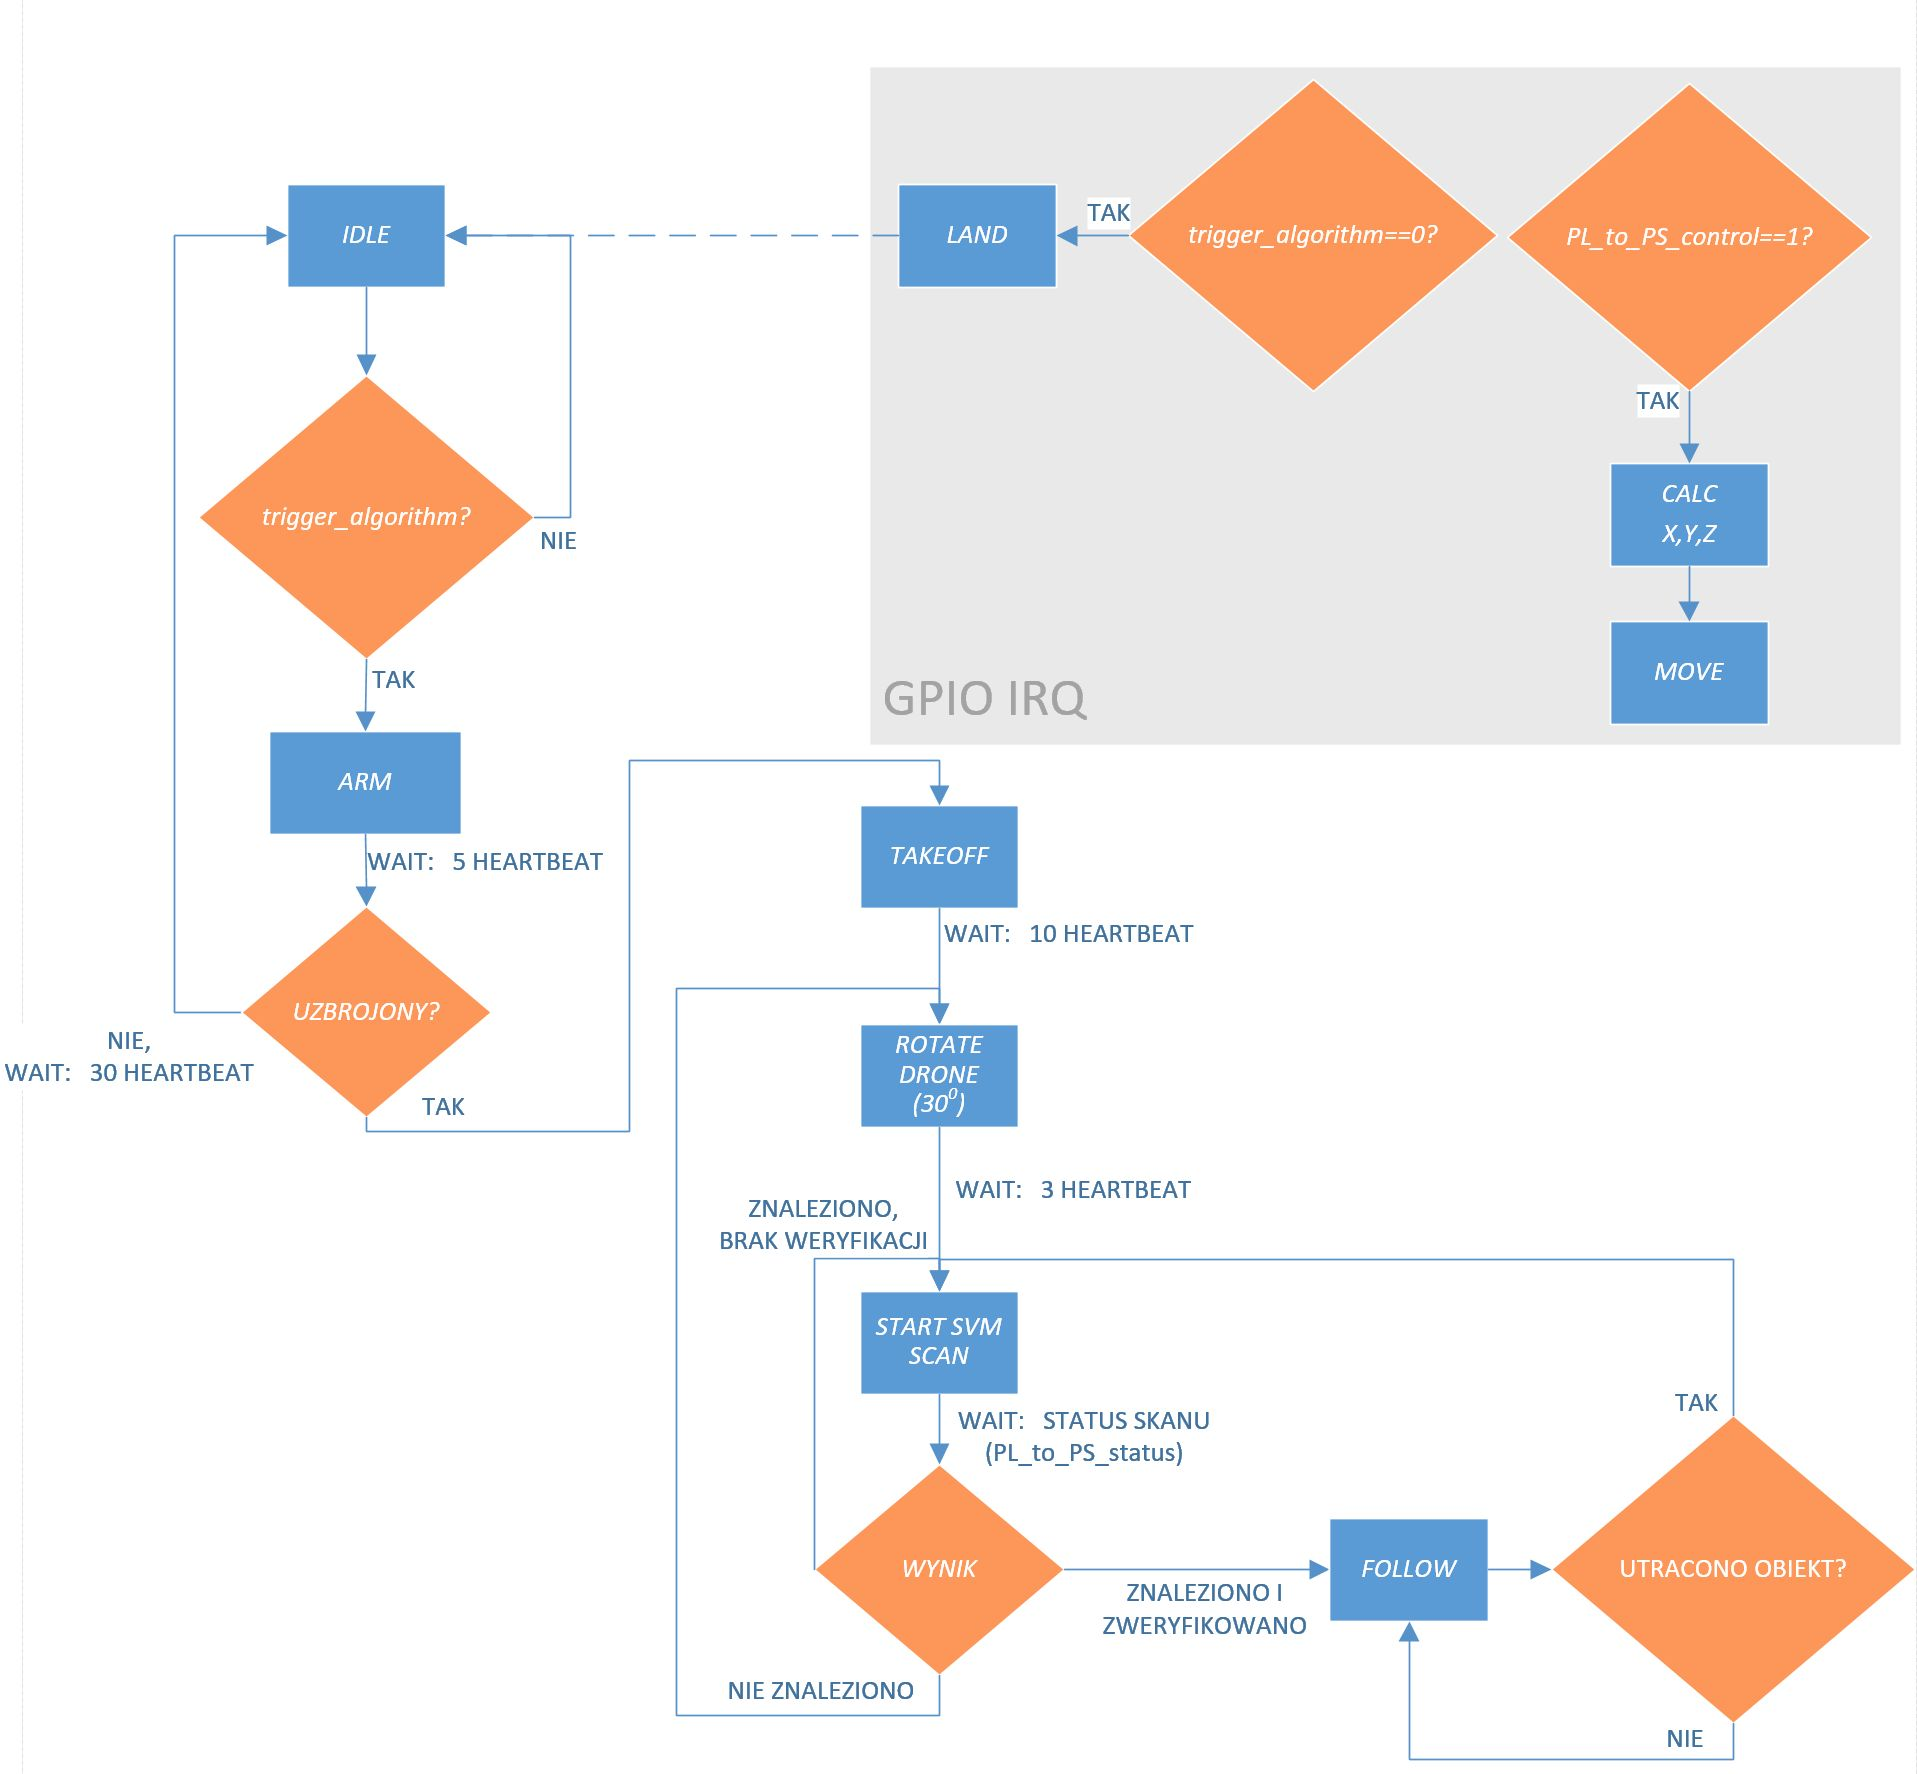
\includegraphics[width=16cm]{5_PS_FSM.jpg}
	\caption{Nadrzędny schemat działania systemu}
	\label{fig:PL_FSM_sch}
\end{figure}

Po otrzymaniu z PL sygnałow sterujących obliczane są przesunięcia (w metrach):
\begin{equation}
\left.\begin{aligned}
x&= \frac{skala_{zadana}-skala}{x_w}\\
y&= \frac{x_{pos}-x_{zadane}}{skala\cdot y_w}\\
z&= \frac{y_{pos}-y_{zadane}}{skala\cdot z_w},\\
\end{aligned}\right.
\end{equation}
gdzie \textit{yPos, xPos, skala} to informacje pochodzące z algorytmów MS/HoG+SVM, a \textit{x_w,y_w,z_w} są empirycznie dobranymi współczynnikami. Warto zwrócić uwagę na zmianę osi układu współrzędnych drona:
\begin{itemize}
	\item \textit{x} - oś pozioma odpowiadająca kierunkowi ruchu samolotu (aspekt głębokości na obrazie),
	\item \textit{y} - oś pozioma prostopadła do osi \textit{x},
	\item \textit{z} - oś pionowa, zwrócona w dół.
\end{itemize}